% !TeX spellcheck = en_GB
\section{Hourly averages ensemble member zero and one}%\hfill} 
\label{app:EM1h}

%%% image 1h %%%%%%%%%%%%%%%%%%%%%%%%%%%%%%%%%%%%%
\begin{figure}[H]%\ContinuedFloat
		\centering
        % 22/12
		\begin{subfigure}[t]{\textwidth}
    \centering
    	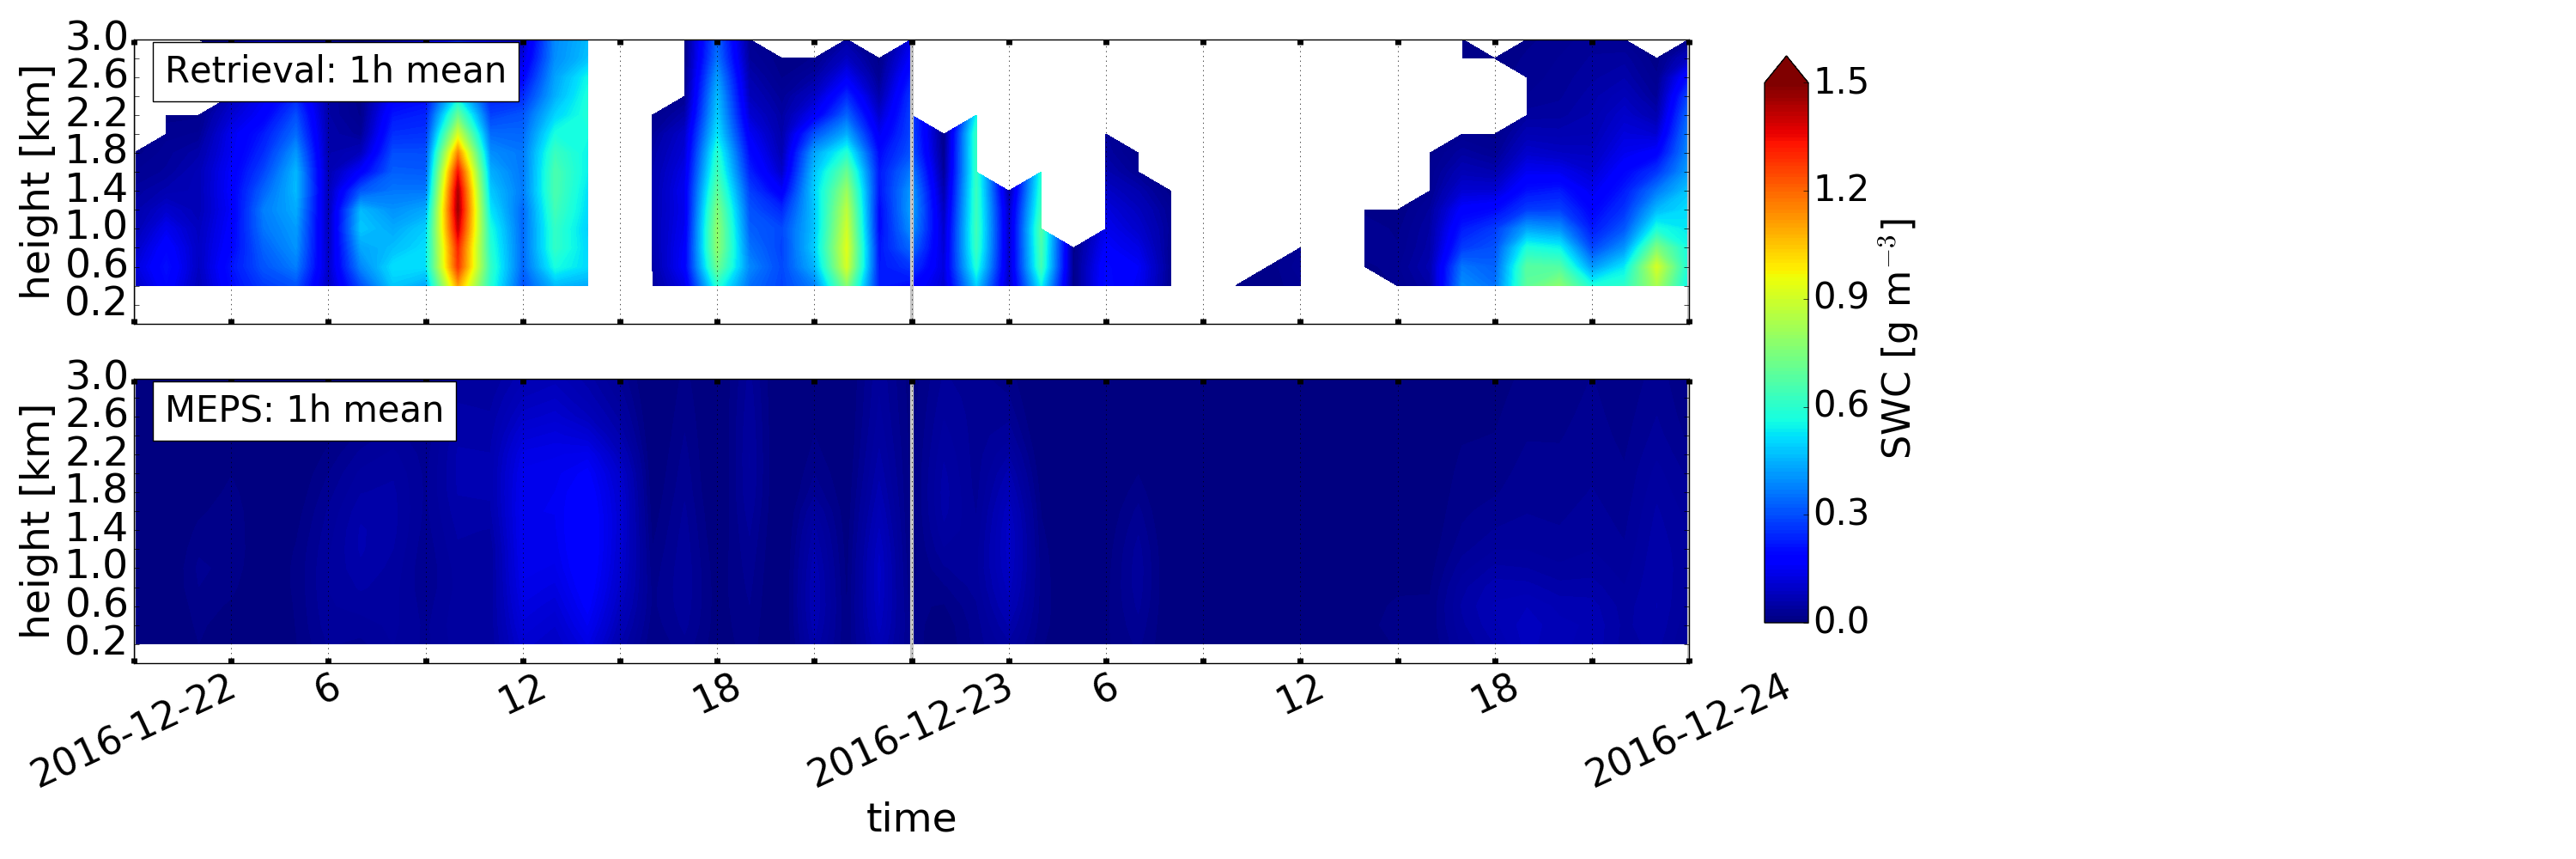
\includegraphics[trim={0.cm 0.8cm 19.cm 0.5cm},clip,width=0.9\textwidth]{./fig_vert_SWC_1h/20161222}
		\caption{}\label{fig:SWC1h:22}
    \end{subfigure}
        % 23/12
		\begin{subfigure}[t]{\textwidth}
    \centering
    	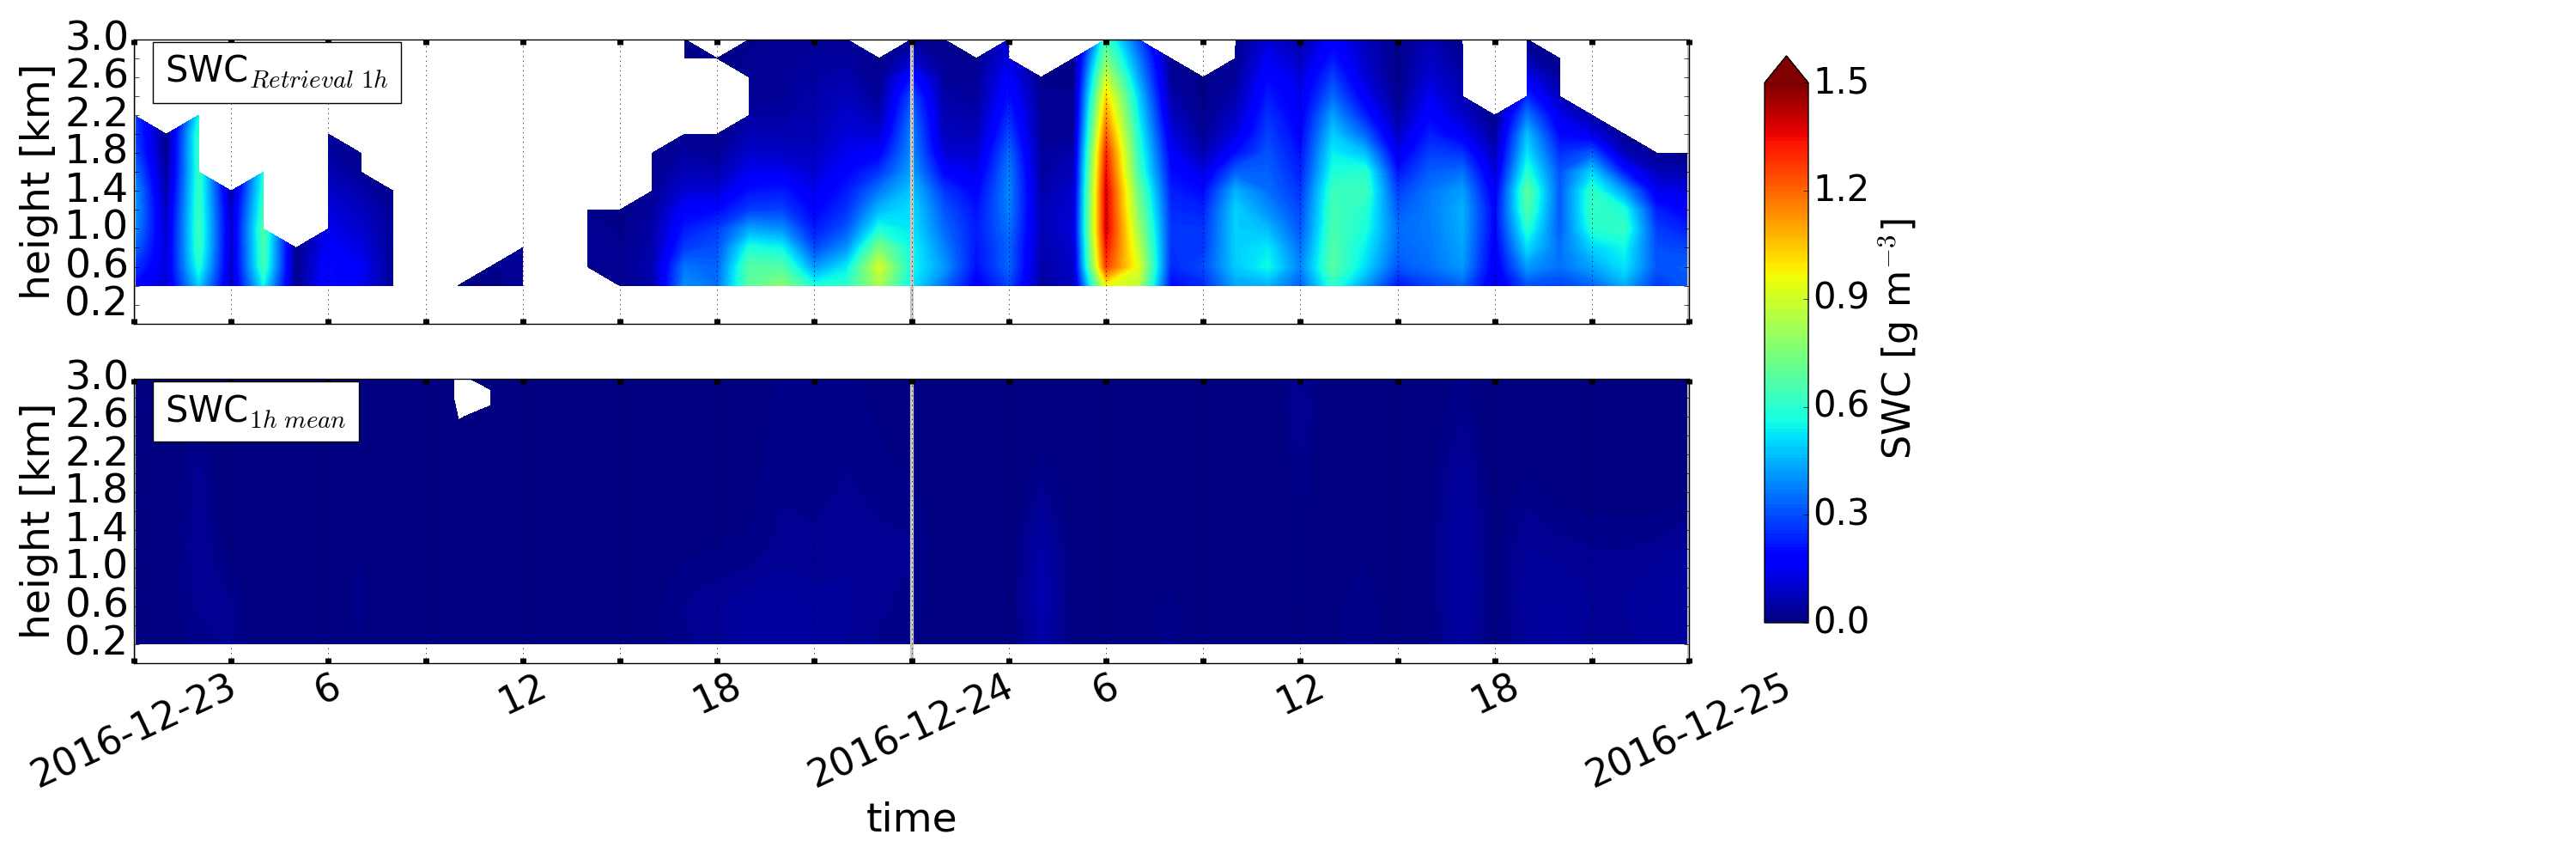
\includegraphics[trim={0.cm 0.8cm 19.cm 0.5cm},clip,width=0.9\textwidth]{./fig_vert_SWC_1h/20161223}
		\caption{}\label{fig:SWC1h:23}
    \end{subfigure}
    \caption{Upper panel: hourly averaged retrieved SWC, lower panel instantaneous hourly averaged SWC forecast of deterministic and first ensemble member. Initialised \SIlist{22;23}{\dec} at \SI{0}{\UTC}. }\label{fig:SWC_1h}
 \end{figure}
 \begin{figure}[t]\ContinuedFloat
    % 25/12
    \centering
		\begin{subfigure}[t]{\textwidth}
    \centering
    	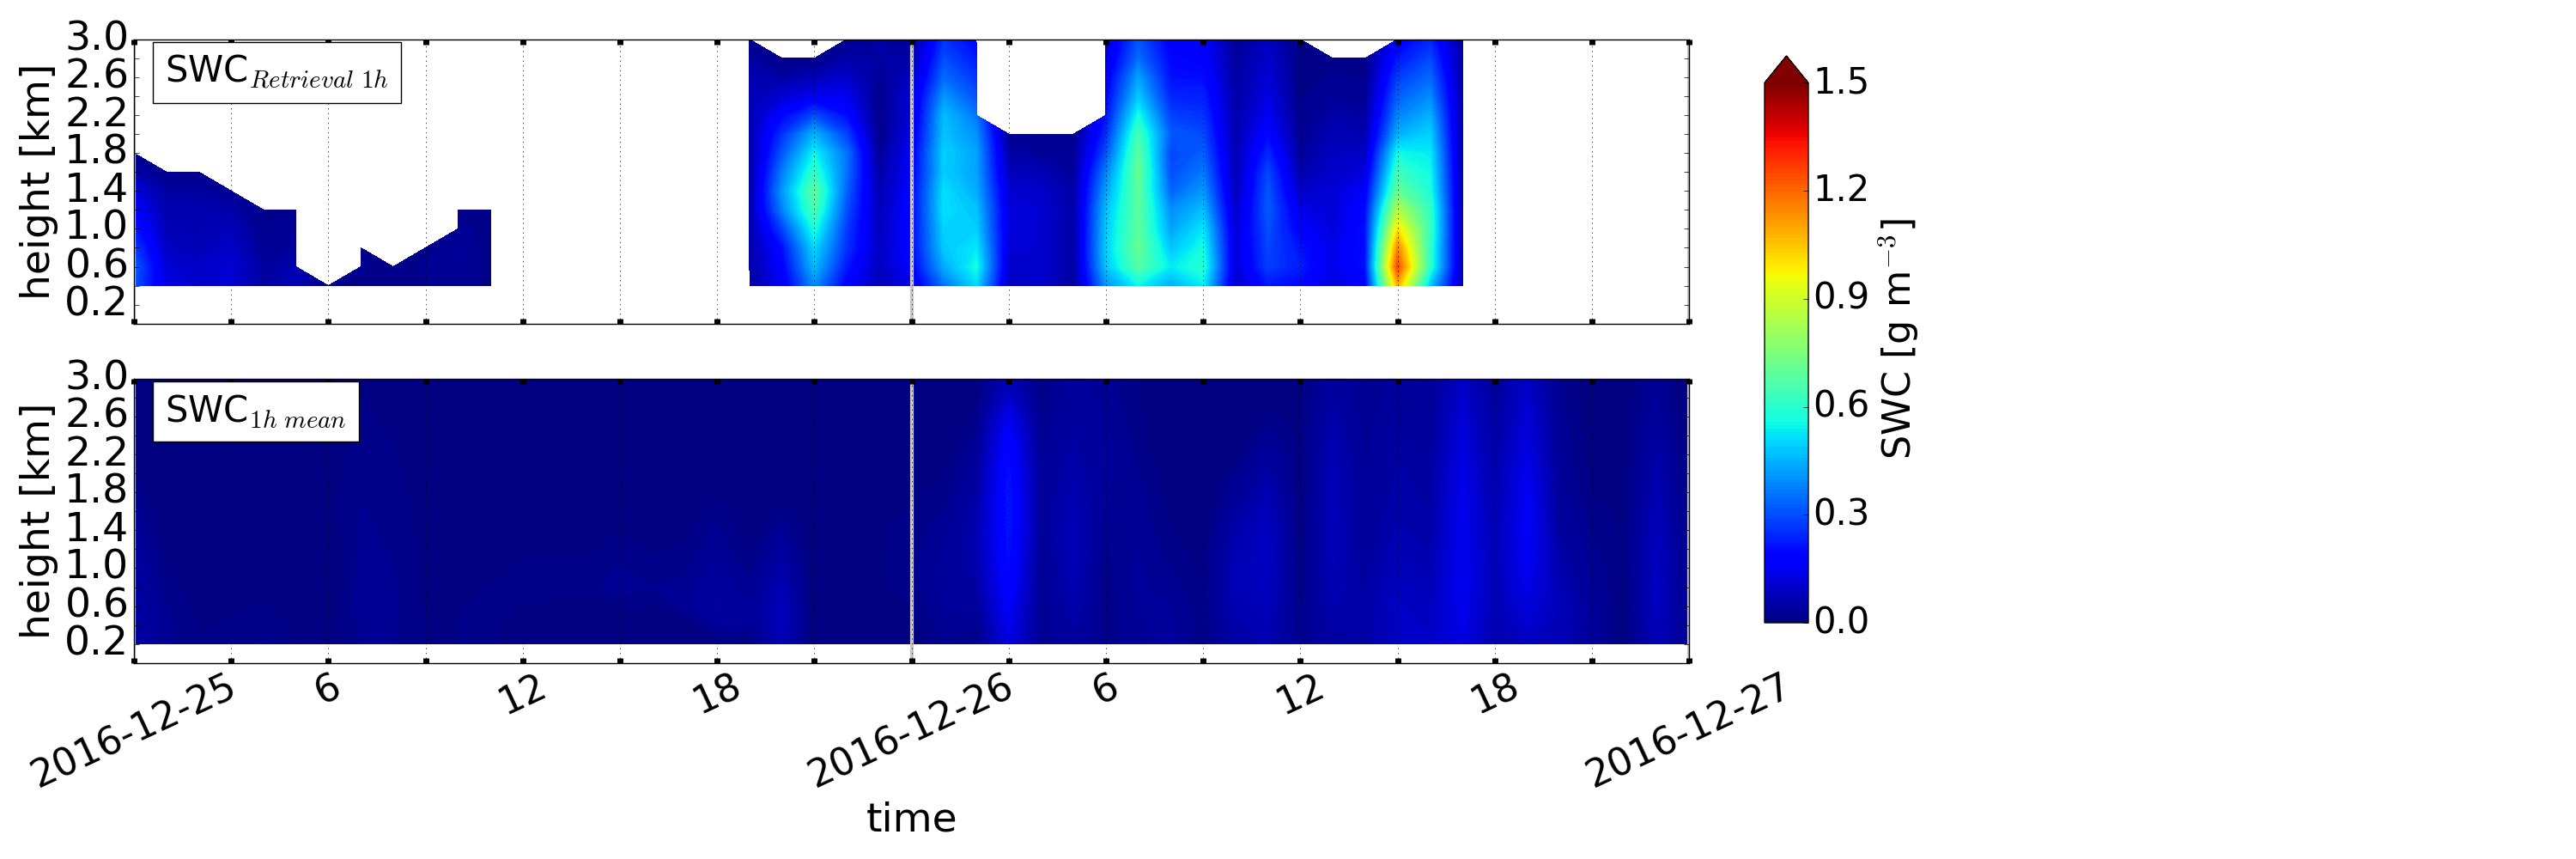
\includegraphics[trim={0.cm 0.8cm 19.cm 0.5cm},clip,width=0.9\textwidth]{./fig_vert_SWC_1h/20161225}
		\caption{}\label{fig:SWC1h:25}
    \end{subfigure}
% \end{figure}
% \begin{figure}[t]\ContinuedFloat
% 	\centering
    % 26/12
		\begin{subfigure}[t]{\textwidth}
    \centering
    	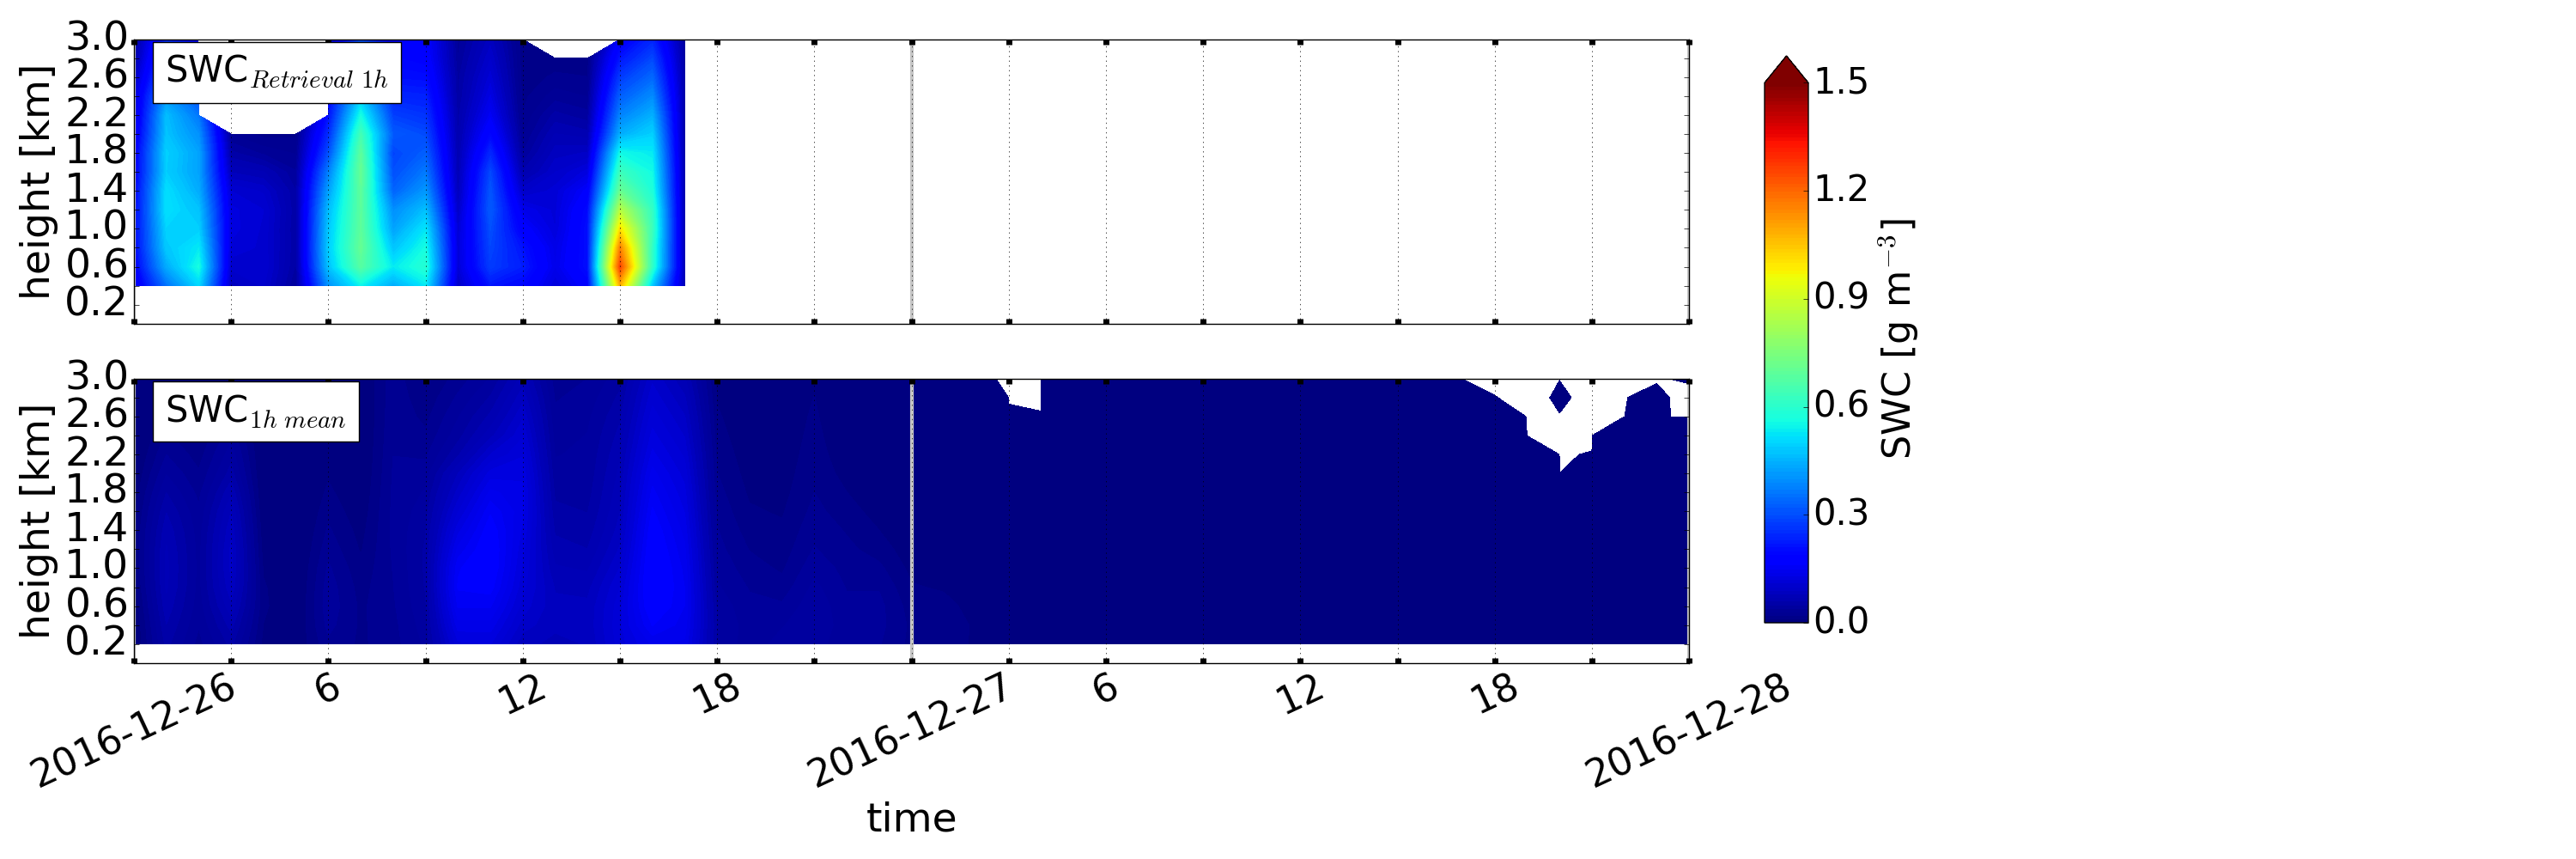
\includegraphics[trim={0.cm 0.8cm 19.cm 0.5cm},clip,width=0.9\textwidth]{./fig_vert_SWC_1h/20161226}
		\caption{}\label{fig:SWC1h:26}
    \end{subfigure}
\caption{\textit{(Continued from previous page.)} Initialised \SIlist{25;26}{\dec} at \SI{0}{\UTC}.}   
\end{figure}
%%%%%%%%%%%%%%%%%%%%%%%%%%%%%%%%%%%%%%%%%%%%%%%%%%%%%%%%%%%%%%%%%%%%%%%%%%
